% =====================================================================
% CHANGELOG (corrected SI). Run hash 0a775ac4f1ead9d3, M=1000.
% Major edits:
%  - S6.2 materiality: clarified beta_min as a single-participant resolution
%    floor (within-participant residual scale); added the normal-equivalent
%    stringency formula with the explicit caveat that it is not a fixed alpha and
%    the confirmatory calibration is design-based.
%  - S8: added the "Scope boundary: endpoint-by-delay collider selection"
%    subsection (mechanism, diagnostics, hard support-blocking rule); updated the
%    worked selection calculation to the realised slope (-60.6) and fixed the
%    Lee/Manski and gate numbers.
%  - S9: behaviours expanded from four to seven; removed the stale beta_min=33;
%    fixed "residual scale" -> endpoint-level injection; added the "Realised
%    operating characteristics" subsection with the design and outcomes tables and
%    the collider sweep, all from the frozen run.
%  - S9 worked example: regenerated from a real supported replicate (#946) and a
%    real null replicate (#514); every decision object now matches the pipeline.
%  - S10 checklist: added code/archive availability (GitHub, Zenodo, run hash).
%  - Converted all \emph to \textit per house style.
% =====================================================================
\documentclass[11pt,a4paper]{article}

\usepackage[top=20mm,bottom=20mm,left=20mm,right=20mm]{geometry}
\usepackage[T1]{fontenc}
\usepackage{setspace}
\onehalfspacing
\usepackage{amsmath,amssymb,amsthm,mathtools}
\usepackage{graphicx}
\usepackage{booktabs}
\usepackage{caption}
\usepackage{float}
\usepackage{array,tabularx}
\usepackage{enumitem}
\usepackage{xcolor}
\usepackage{authblk}
\usepackage[super,sort&compress]{natbib}
\usepackage[colorlinks,citecolor=blue!60!black,linkcolor=blue!60!black,
            urlcolor=blue!60!black]{hyperref}
\usepackage{cleveref}
\usepackage{xurl}
\usepackage{pifont}
\usepackage{tikz}
\usetikzlibrary{arrows.meta,positioning,calc,fit,backgrounds}

\newtheorem{proposition}{Proposition}
\newtheorem{lemma}{Lemma}
\theoremstyle{definition}
\newtheorem{definition}{Definition}

\newcommand{\F}{\mathcal{F}}
\newcommand{\Apre}{A_{\mathrm{pre}}}
\newcommand{\tauL}{\tau_L}
\newcommand{\UCB}{\mathrm{UCB}_{0.95}}
\newcommand{\LCB}{\mathrm{LCB}_{0.95}}

% number SI floats and equations with an S prefix
\renewcommand{\thesection}{S\arabic{section}}
\renewcommand{\thesubsection}{S\arabic{section}.\arabic{subsection}}
\renewcommand{\theequation}{S\arabic{equation}}
\renewcommand{\thefigure}{S\arabic{figure}}
\renewcommand{\thetable}{S\arabic{table}}
\renewcommand{\theproposition}{S\arabic{proposition}}
\renewcommand{\thelemma}{S\arabic{lemma}}

\title{\textbf{Electronic Supplementary Material\\[4pt]
Testing past-adapted accounts of anticipatory EEG\\[4pt] with post-endpoint randomisation}}

\author[1]{George Sopasakis}
\author[2]{Alexandros Sopasakis}
\affil[1]{Research and Development Department, Ximantis AB, Onsala, Sweden}
\affil[2]{Department of Mathematics, Lund University, Lund, Sweden}
\date{\today}

\begin{document}
\maketitle

\noindent
This supplement gives the formal and operational detail behind the
post-endpoint randomisation test described in the main text. It supports the
Level~II-A design only. It contains no mechanistic, dynamical, or physical model
of any residual; the construction and evaluation of such models are separate,
prospectively specified work. Section numbering uses an \textbf{S} prefix and is
self-contained. All references to ``the main text'' point to the accompanying
Perspective.

\tableofcontents
\bigskip

% =====================================================================
\section{Formal randomisation boundary}
\label{sec:si-randomisation-boundary}

This section proves the conditional-exclusion result stated as
Proposition~1 in the main text and records the measure-theoretic conditions it
needs. The result is elementary; we give it in full because the entire
evidential logic of the design rests on it.

\subsection{Setup and filtration}
\label{sec:si-filtration}

Fix a trial \(j\) with randomisation stratum \(\mathcal{R}_j\) and committed
endpoint window \(I_{\mathrm{pre}}=[t_0,t_1]\). Let
\((\Omega,\mathcal{A},\mathbb{P})\) carry the trial process, and let
\(\{\F_t^{(j)}\}_{t\le t_1}\) be the filtration generated by all
pre-assignment information: neural and physiological history, protocol state,
elapsed foreperiod, conditional hazard, arousal and vigilance proxies,
motor-preparation proxies, block and session state, time on task, and
previous-trial variables. The stratum label \(\mathcal{R}_j\) is
\(\F_{t_1}^{(j)}\)-measurable. The assigned delay
\(\tauL^{(j)}\in[0,T_0]\) is generated after \(t_1\) by an independent service
with declared conditional law
\(P_{\mathrm{sch}}(\mathrm{d}\tauL\mid\mathcal{R}_j)\).

\begin{definition}[Past-adapted statistic]
\label{def:past-adapted}
A real-valued statistic \(X^{(j)}\) is past-adapted on trial \(j\) if it is
\(\F_{t_1}^{(j)}\)-measurable, i.e. computable from information available at or
before \(t_1\).
\end{definition}

\begin{definition}[Exogenous post-endpoint randomisation]
\label{def:exogenous}
The randomisation source is exogenous if, conditional on \(\mathcal{R}_j\), the
assigned delay is independent of the pre-assignment history,
\begin{equation}
\label{eq:si-exogeneity}
\tauL^{(j)}\ \perp\!\!\!\perp\ \F_{t_1}^{(j)}\ \mid\ \mathcal{R}_j .
\end{equation}
\end{definition}

Equation~\eqref{eq:si-exogeneity} is the formal content of condition~(R1) under
the past-adapted null. It is an assumption about the assignment mechanism, made
plausible by concealment and post-endpoint generation and tested by the
randomisation, leakage, and implementation-swap audits of
\Cref{sec:si-leakage-controls}. It is not established by inspecting the
assignment software.

\subsection{Conditional exclusion}
\label{sec:si-exclusion-proof}

\begin{proposition}[Conditional exclusion of the past-adapted class]
\label{prop:si-exclusion}
Let \(X^{(j)}\) be integrable, \(\mathbb{E}\lvert X^{(j)}\rvert<\infty\).
\begin{enumerate}[leftmargin=2.0em,itemsep=2pt]
\item If \(X^{(j)}\) is past-adapted and \eqref{eq:si-exogeneity} holds, then
\begin{equation}
\label{eq:si-fwd-null}
\mathbb{E}\!\left[X^{(j)}\mid\sigma(\tauL^{(j)}),\mathcal{R}_j\right]
=\mathbb{E}\!\left[X^{(j)}\mid\mathcal{R}_j\right]\quad\text{a.s.},
\end{equation}
and for every Borel \(B\) with
\(P_{\mathrm{sch}}(B\mid\mathcal{R}_j)>0\),
\(\mathbb{E}[X^{(j)}\mid\tauL^{(j)}\in B,\mathcal{R}_j]
=\mathbb{E}[X^{(j)}\mid\mathcal{R}_j]\).
\item Equation~\eqref{eq:si-fwd-null} applies with \(X^{(j)}=\Apre^{(j)}\) and
with any prospectively fixed transform \(g(\Apre^{(j)})\) whose parameters do not
depend on the assignment vector, provided \(\Apre^{(j)}\) is past-adapted, which
holds under conditions~(R1)--(R2).
\item Under (R1)--(R3), \eqref{eq:si-fwd-null} extends to the retained analysis
sample only if retention, delivery, preprocessing, missingness, and inclusion
preserve the randomised contrast; \Cref{sec:si-sensitivity-analysis} makes this
condition operational.
\end{enumerate}
\end{proposition}

\begin{proof}
For part~1, since \(X^{(j)}\) is \(\F_{t_1}^{(j)}\)-measurable and, by
\eqref{eq:si-exogeneity}, \(\tauL^{(j)}\) is conditionally independent of
\(\F_{t_1}^{(j)}\) given \(\mathcal{R}_j\), the pair
\((X^{(j)},\mathcal{R}_j)\) is conditionally independent of \(\tauL^{(j)}\) given
\(\mathcal{R}_j\). Hence for any bounded measurable \(\phi\),
\(\mathbb{E}[X^{(j)}\phi(\tauL^{(j)})\mid\mathcal{R}_j]
=\mathbb{E}[X^{(j)}\mid\mathcal{R}_j]\,\mathbb{E}[\phi(\tauL^{(j)})\mid\mathcal{R}_j]\).
Taking \(\phi=\mathbf{1}_B\) and dividing by
\(P_{\mathrm{sch}}(B\mid\mathcal{R}_j)>0\) gives the stated set equality; the
conditional-expectation form \eqref{eq:si-fwd-null} follows by the defining
property of conditional expectation given \(\sigma(\tauL^{(j)})\vee\mathcal{R}_j\)
and a monotone-class argument extending from indicators to integrable \(X^{(j)}\).
Part~2 is the special case \(X^{(j)}=\Apre^{(j)}\) (or
\(X^{(j)}=g(\Apre^{(j)})\)); under (R2) the endpoint and any fixed transform are
past-adapted because confirmatory preprocessing is strictly causal and
label-blind. Part~3 fails in general once selection acts after assignment: if an
inclusion indicator \(S^{(j)}\) depends on both \(\Apre^{(j)}\) and
\(\tauL^{(j)}\), then conditioning on \(S^{(j)}=1\) can induce dependence even
when \eqref{eq:si-fwd-null} holds marginally. The magnitude of this induced
dependence is bounded in \Cref{sec:si-sensitivity-analysis}.
\end{proof}

\subsection{Scope of the statement}
\label{sec:si-scope}

Proposition~\ref{prop:si-exclusion} is a boundary statement, not a sufficiency
theorem for the comparator. It says only that a past-adapted statistic cannot be
ordered by a post-endpoint assigned delay under \eqref{eq:si-exogeneity}. It does
not assert that the forward-only comparator has captured every neural cause of
anticipation. Identification of the delay contrast comes from the randomisation
mechanism, not from the completeness of any covariate set. A material
delay ordering of the committed endpoint therefore localises to one of:
(i) failure of \eqref{eq:si-exogeneity} (randomisation or concealment failure);
(ii) failure of past-adaptedness of the endpoint or a comparator covariate
(temporal leakage, condition~(R2)); (iii) a post-randomisation selection pathway
(condition~(R3)); or (iv) the declared past-adapted account being conditionally
insufficient in the tested regime. The audits and sensitivity analysis are built
to separate (i)--(iii) from (iv).

% =====================================================================
\section{Endpoint definition and preprocessing lock}
\label{sec:si-endpoint-preprocessing}

\subsection{Locked endpoint specification}
\label{sec:si-endpoint-spec}

The committed endpoint \(\Apre^{(j)}\) is a single-trial, signed,
baseline-corrected scalar feature. Before any delay label is accessed, the
protocol locks the components in \Cref{tab:si-endpoint-lock}. Once locked, these
are irrevocable for confirmatory analysis; changes define a new regime and
require a new protocol.

\begin{table}[t]
\centering
\caption{Locked components of the committed pre-event endpoint and comparator.}
\label{tab:si-endpoint-lock}
\footnotesize
\begin{tabularx}{\textwidth}{@{}p{3.4cm}X@{}}
\toprule
\textbf{Component} & \textbf{Locked information} \\
\midrule
Recording & Modality, sampling rate, channel or source set, montage, reference,
online filters (causal only). \\
Endpoint window & \(I_{\mathrm{pre}}=[t_0,t_1]\) relative to the warning cue;
baseline interval; closing time \(t_1\). \\
Feature & Temporal operation (e.g.\ mean slope or window average), aggregation
rule across channels, sign convention. \\
Eligibility & Trial-inclusion and artefact criteria computable from
\(\F_{t_1}^{(j)}\); rejection thresholds. \\
Comparator covariates & Past-adapted covariate vector \(X_j\)
(\Cref{tab:si-comparator}); transforms and interactions. \\
Folds and loss & Cross-fitting fold structure (block-respecting); comparator
family, tuning rule, loss. \\
Decision constants & Materiality threshold \(\beta_{\min}\); \(N_{\min}\);
randomisation-replicate count; bootstrap settings. \\
\bottomrule
\end{tabularx}
\end{table}

\subsection{Strict causality and the preprocessing lock}
\label{sec:si-causality}

Every confirmatory operation that directly produces the endpoint or a comparator
covariate is strictly causal: an output at time \(t\le t_1\) depends only on
samples at \(u\le t\). The following are prohibited for confirmatory endpoint
construction: zero-phase, bidirectional, forward--reverse, symmetric, and
time-shift-corrected filtering; baseline or detrending steps that use
post-\(t_1\) samples; and any preprocessing, rejection, or inclusion rule that
depends on the delay label.

Label-blind artefact models are allowed only as nuisance procedures under the
same endpoint-lock constraint. Their training data, application window, and
rejection rules must be fixed before delay access, and the temporal-leakage audit
must show that post-\(t_1\) activity cannot change the committed endpoint beyond
the declared tolerance. Any acausal pipeline that fails this requirement may be
reported only as an exploratory robustness analysis, clearly separated from the
confirmatory result.

\subsection{Temporal-leakage audit}
\label{sec:si-leakage-audit}

Before delay labels are accessed, the complete locked endpoint-and-comparator
pipeline is applied to synthetic audit records that are flat over
\(I_{\mathrm{pre}}\) and carry controlled post-\(t_1\) content: impulses, step
responses, and event-locked transients placed at the earliest and latest
admissible delivered latencies. The pipeline passes only if these post-endpoint
inputs produce no committed pre-event output beyond a declared tolerance
\(\delta_{\mathrm{leak}}\), fixed prospectively as a small fraction of the
endpoint's label-blind noise scale. Failure invalidates the confirmatory endpoint
irrespective of any later slope. \Cref{fig:si-lock} shows the ordering of the
lock and the barrier it creates.

\begin{figure}[t]
\centering
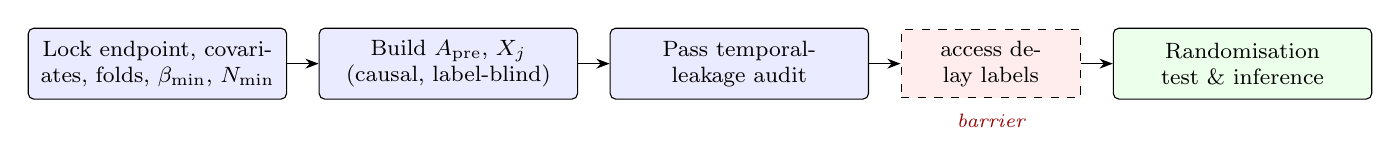
\begin{tikzpicture}[>=Stealth,font=\footnotesize,node distance=4mm,
  blind/.style={draw,rounded corners=2pt,fill=blue!8,align=center,
                text width=3.0cm,minimum height=0.9cm,inner sep=4pt},
  conf/.style={draw,rounded corners=2pt,fill=green!8,align=center,
               text width=3.0cm,minimum height=0.9cm,inner sep=4pt},
  bar/.style={draw,dashed,fill=red!7,align=center,text width=2.0cm,inner sep=4pt}]
\node[blind] (spec) {Lock endpoint, covariates, folds, $\beta_{\min}$, $N_{\min}$};
\node[blind,right=of spec] (build) {Build $\Apre$, $X_j$ (causal, label-blind)};
\node[blind,right=of build] (leak) {Pass temporal-leakage audit};
\node[bar,right=of leak] (barrier) {access delay labels};
\node[conf,right=of barrier] (test) {Randomisation test \& inference};
\draw[->] (spec)--(build); \draw[->] (build)--(leak); \draw[->] (leak)--(barrier);
\draw[->] (barrier)--(test);
\node[below=2pt of barrier,font=\scriptsize\itshape,text=red!60!black]{barrier};
\end{tikzpicture}
\caption{Endpoint and preprocessing lock. All construction occurs label-blind and
must pass the temporal-leakage audit before delay labels are accessed.}
\label{fig:si-lock}
\end{figure}

% =====================================================================
\section{Forward-only comparator specification}
\label{sec:si-forward-comparator}

\subsection{Covariate class}
\label{sec:si-covariates}

The forward-only comparator absorbs known anticipatory structure. Its covariates are
listed in \Cref{tab:si-comparator}. Every covariate must be
\(\F_{t_1}^{(j)}\)-measurable. No realised-delay label, and no deterministic
transform of one, may enter comparator fitting. Covariates derived from scheduler
state are admissible only insofar as they are known before \(t_1\) (e.g.\ block
probabilities, elapsed foreperiod), not the specific post-endpoint draw.

\begin{table}[t]
\centering
\caption{Forward-only comparator covariate class. All entries are past-adapted
(\(\F_{t_1}^{(j)}\)-measurable).}
\label{tab:si-comparator}
\footnotesize
\begin{tabularx}{\textwidth}{@{}p{3.6cm}X@{}}
\toprule
\textbf{Group} & \textbf{Covariates} \\
\midrule
Timing & Elapsed foreperiod; conditional hazard; scheduler/block probability
known pre-\(t_1\). \\
Slow potential & CNV-like slow-potential amplitude or slope over a pre-\(t_1\)
window disjoint from the endpoint feature. \\
State & Arousal/vigilance proxy (e.g.\ pupil or alpha-band measure);
motor-preparation proxy. \\
History & Previous-trial timing and outcome; reaction-time history; sequential
indices; time on task. \\
Structure & Participant and session identifiers; preprocessing covariates
(e.g.\ retained-channel counts). \\
Interactions & Prospectively declared interactions and nonlinear transforms of
the above. \\
\bottomrule
\end{tabularx}
\end{table}

\subsection{Family, cross-fitting and the frozen residual}
\label{sec:si-crossfit}

The comparator family may be high-capacity (penalised regression, gradient
boosting, random forests, or recurrent/state-space predictors), with family,
tuning rule, fold structure, and loss locked before delay access. Outer
cross-fitting folds are fixed prospectively and keep randomisation blocks intact;
all hyperparameter selection occurs inside the corresponding training partition.
For a trial in fold \(k(j)\),
\begin{equation}
\label{eq:si-residual}
\Apre^{\mathrm{resid},(j)}
=\Apre^{(j)}-\widehat{m}_0^{\,(-k(j))}(X_j),
\qquad
\widehat{m}_0^{\,(-k)}\approx\mathbb{E}[\Apre\mid X,\ \text{folds}\ne k].
\end{equation}
Held-out predictions and residuals are generated once and frozen before the
randomisation test. Refitting or retuning inside the test loop is prohibited.

\subsection{Why residualisation does not identify the contrast}
\label{sec:si-design-based}

Residualisation improves precision and tests robustness against conventional
explanations, but it is not the source of identification. The delay contrast is
identified by the assignment mechanism. This matters for validity because a
flexible nuisance fit can borrow endpoint information across trials, so the fitted
residual \(\Apre^{\mathrm{resid},(j)}\) is not focal-trial measurable. The
randomisation test therefore holds the entire frozen residual array fixed and
regenerates only the assigned-delay vector, under the assignment mechanism
actually used.
This follows covariate-adjusted randomisation-inference logic
\citep{ZhaoDing2021}, extended to cross-fitting compatible with the
randomisation design rather than an i.i.d.\ sampling approximation
\citep{LuEtAl2025}. Holding
all endpoints fixed under reassignment is exact only under a sharp null that also
excludes carryover of \(\tauL^{(j)}\) to later endpoints; when carryover is
possible the sequential-score route of \Cref{sec:si-estimand-inference} is used.

% =====================================================================
\section{Confirmatory estimand and inference}
\label{sec:si-estimand-inference}

\subsection{Participant-level estimand}
\label{sec:si-estimand}

Within participant \(p\), trial \(j\), stratum \(\mathcal{R}_{pj}\), with the
assigned delay centred at its scheduler mean
\(\bar\tau_{\mathcal{R}_{pj}}=\mathbb{E}_{P_{\mathrm{sch}}}[\tauL\mid\mathcal{R}_{pj}]\),
\begin{equation}
\label{eq:si-participant-slope}
\Apre^{\mathrm{resid},(pj)}
=\alpha_{\mathcal{R}_{pj}}
+\beta_{\tau,p}\bigl(\tauL^{(pj)}-\bar\tau_{\mathcal{R}_{pj}}\bigr)
+\varepsilon_{pj},
\qquad
\beta_\tau=\mathbb{E}_p[\beta_{\tau,p}].
\end{equation}
Each eligible participant contributes one slope, with equal weight. A
prospectively fixed rule handles any non-estimable participant identically in
every replicate.

\subsection{Intention-to-treat indexing}
\label{sec:si-itt}

The primary analysis is indexed by the assigned label \(\tauL^{(j)}\), the
quantity protected by randomisation, not by the measured latency
\(\widetilde{\tau}_L^{(j)}=t_{\mathrm{event}}^{(j)}-t_1\). This preserves the
randomisation guarantee under operating-system jitter, display or audio latency,
dropped frames, or trigger delay. The measured latency is retained for the
delivery audit (\Cref{sec:si-leakage-controls}) and for descriptive
compliance reporting only.

\subsection{Sequential-score route under carryover}
\label{sec:si-sequential}

When the delay assigned on trial \(j\) may affect the endpoint on later trials,
the assignment-isolation sharp null is not exact. The default in that case is the
sequential-score route. The current endpoint and residual are treated as part of
the pre-assignment history for the current draw, and the participant slope is the
estimating-equation coefficient
\begin{equation}
\label{eq:si-sequential-slope}
\widehat{\beta}_{\tau,p}^{\,\mathrm{seq}}
=\frac{\sum_{j\in\mathcal{J}_p}\Apre^{\mathrm{resid},(pj)}\,\Delta\tau_{pj}}
       {\sum_{j\in\mathcal{J}_p}v_{pj}},
\qquad
\Delta\tau_{pj}=\tauL^{(pj)}-\bar\tau_{\mathcal{R}_{pj}},
\end{equation}
with \(v_{pj}=\operatorname{Var}_{P_{\mathrm{sch}}}(\tauL\mid\mathcal{R}_{pj})\)
the per-trial assignment variance. The centred increment
\(\Delta\tau_{pj}\) is a martingale difference with respect to the
pre-assignment history under \eqref{eq:si-exogeneity}, so
\(\sum_j\Apre^{\mathrm{resid},(pj)}\Delta\tau_{pj}\) has conditional mean zero
under the null; the corresponding conditional-randomisation calibration is given
in \Cref{sec:si-randomisation-test}. The assignment-isolation route is permitted
only when predeclared reset or washout diagnostics (lagged
endpoint-on-previous-delay checks, pass thresholds, minimum retained-trial yield,
and required delay leverage) justify endpoint-array invariance; failure reverts to
the sequential-score route or classifies the study as operationally unqualified.

% =====================================================================
\section{Randomisation test}
\label{sec:si-randomisation-test}

\subsection{Assignment-isolation route}
\label{sec:si-iso-route}

The test statistic is the equal-participant average slope
\(\widehat{\beta}_\tau=\frac1P\sum_p\widehat{\beta}_{\tau,p}\) computed from the
frozen residuals. The sharp null states that each committed residual is invariant
to admissible reassignment of \(\tauL\). Each replicate reproduces the assignment
mechanism actually used: fixed multisets are permuted within their declared
blocks, and stochastic draws are redrawn from
\(P_{\mathrm{sch}}(\mathrm{d}\tauL\mid\mathcal{R}_{pj})\). No replicate moves an
assignment across participant, session, block, or other declared stratum, and the
frozen residual array is never recomputed.

\subsection{One-sided \texorpdfstring{$p$}{p}-value}
\label{sec:si-pvalue}

Let \(\widehat{\beta}_\tau^{(r)}\), \(r=1,\dots,R\), be the replicate statistics.
The one-sided randomisation \(p\)-value, with the finite-sample plus-one
correction, is
\begin{equation}
\label{eq:si-pvalue}
p_{\mathrm{rand}}
=\frac{1+\#\{r:\widehat{\beta}_\tau^{(r)}\le\widehat{\beta}_\tau\}}{1+R}.
\end{equation}
The number of replicates \(R\) is declared prospectively. Where exhaustive
enumeration is feasible it replaces the Monte Carlo estimate. The
assignment-calibrated criterion passes when \(p_{\mathrm{rand}}\le\alpha\) for the
declared one-sided level \(\alpha\) \citep{Harris2023}.

\subsection{Sequential-score calibration}
\label{sec:si-seq-calibration}

Under the sequential-score route, the statistic
\(T_p=\sum_{j}\Apre^{\mathrm{resid},(pj)}\Delta\tau_{pj}\) is calibrated against
its conditional-randomisation distribution. Each replicate conditions on the
observed pre-assignment histories and redraws the current-trial assigned delays
from the declared scheduler within the corresponding strata; the centred
contrasts \(\Delta\tau_{pj}\) are then recomputed using the same centring rule as
in \Cref{eq:si-sequential-slope}. The residuals are not recomputed. This
calibration tests whether the observed martingale-score sum is unusually
negative under conditionally random assignment, without assuming that later
endpoints would remain unchanged under a counterfactual reassignment of earlier
trials.

The observed aggregate statistic
\[
T_{\mathrm{seq}}
=
\frac{\sum_p T_p}{\sum_p\sum_{j\in\mathcal{J}_p} v_{pj}}
\]
is compared with the corresponding replicate statistics using
\eqref{eq:si-pvalue}, with \(v_{pj}\) defined as the scheduler variance in
\Cref{eq:si-sequential-slope}. \Cref{fig:si-randtest} summarises the workflow.

\begin{figure}[t]
\centering
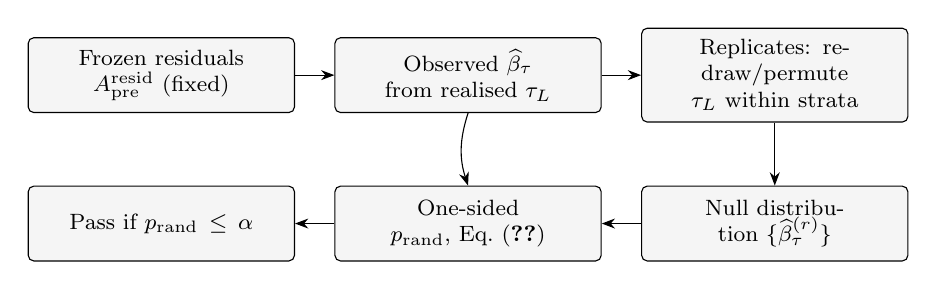
\begin{tikzpicture}[>=Stealth,font=\footnotesize,node distance=5mm,
  s/.style={draw,rounded corners=2pt,fill=gray!8,align=center,
            text width=3.1cm,minimum height=0.95cm,inner sep=4pt}]
\node[s] (frozen) {Frozen residuals $\Apre^{\mathrm{resid}}$ (fixed)};
\node[s,right=of frozen] (obs) {Observed
  $\widehat\beta_\tau$ from realised $\tauL$};
\node[s,right=of obs] (rep) {Replicates: redraw/permute $\tauL$ within strata};
\node[s,below=8mm of rep] (null) {Null distribution
  $\{\widehat\beta_\tau^{(r)}\}$};
\node[s,left=of null] (pv) {One-sided
  $p_{\mathrm{rand}}$, Eq.~\eqref{eq:si-pvalue}};
\node[s,left=of pv] (out) {Pass if
  $p_{\mathrm{rand}}\le\alpha$};
\draw[->] (frozen)--(obs); \draw[->] (obs)--(rep); \draw[->] (rep)--(null);
\draw[->] (null)--(pv); \draw[->] (pv)--(out);
\draw[->] (obs.south) to[bend right=18] (pv.north);
\end{tikzpicture}
\caption{Randomisation-test workflow. The frozen residual array is fixed; only
the assigned-delay vector is regenerated under the declared assignment
mechanism.}
\label{fig:si-randtest}
\end{figure}

\subsection{Finite-sample validity and choice of replicate count}
\label{sec:si-pvalue-finite}

The plus-one randomisation \(p\)-value of \eqref{eq:si-pvalue} is exactly valid in
finite samples, not only asymptotically. Under the sharp null the observed
statistic and the \(R\) replicate statistics are exchangeable, so the rank of the
observed value among the \(R+1\) values is uniform on \(\{1,\dots,R+1\}\). Hence
\begin{equation}
\label{eq:si-pvalue-superuniform}
\mathbb{P}\!\left(p_{\mathrm{rand}}\le\tfrac{k}{R+1}\right)=\tfrac{k}{R+1},
\quad k=1,\dots,R+1,
\qquad\Longrightarrow\qquad
\mathbb{P}\!\left(p_{\mathrm{rand}}\le\alpha\right)\le\alpha
\end{equation}
for every \(\alpha\in(0,1)\) and every finite \(R\) \citep{PhipsonSmyth2010}. The
\(+1\) in numerator and denominator is what makes the test valid rather than
anti-conservative; omitting it admits an impossible \(p=0\) and breaks the level.
This finite-sample exactness, inherited from the assignment mechanism rather than
from a large-sample approximation, is the reason the design uses randomisation
inference for the confirmatory test.

Two finite-\(R\) considerations then fix the replicate count, declared
prospectively. First, granularity: the smallest attainable value is
\(p_{\min}=1/(R+1)\), so \(R\) must satisfy \(p_{\min}<\alpha\) with margin to
resolve the decision; with \(R=9{,}999\), \(p_{\min}=1.0\times10^{-4}\). Second,
Monte Carlo error: \(p_{\mathrm{rand}}\) estimates the ideal
exhaustive-enumeration value \(p^\star\) as a binomial proportion, with
\begin{equation}
\label{eq:si-pvalue-mc-se}
\widehat{\mathrm{se}}(p_{\mathrm{rand}})\approx
\sqrt{\frac{p^\star\,(1-p^\star)}{R}} .
\end{equation}
Near a decision boundary \(p^\star\approx\alpha\) the count \(R\) is set so this
standard error is small relative to \(\alpha\); for \(\alpha=0.05\) and
\(R=9{,}999\), \(\widehat{\mathrm{se}}\approx2.2\times10^{-3}\), about \(4\%\) of
\(\alpha\). The same \(R\) is used in every calibration, including the
\(N_{\min}\) and adversarial-null simulations, so that all reported operating
characteristics share one Monte Carlo resolution. Where the admissible
reassignment set is small enough, exhaustive enumeration removes
\eqref{eq:si-pvalue-mc-se} entirely and is preferred.

% =====================================================================
\section{Participant-level bootstrap and materiality threshold}
\label{sec:si-bootstrap-materiality}

\subsection{Studentised participant bootstrap}
\label{sec:si-bootstrap}

The materiality bound uses a studentised participant bootstrap-\(t\). Resample
participants with replacement, carrying all of each participant's trials,
sessions, strata, and frozen residuals intact; recompute
\(\widehat{\beta}_\tau^{*}\) and its participant-level standard error
\(\widehat{\mathrm{se}}^{*}\); and form
\(t^{*}=(\widehat{\beta}_\tau^{*}-\widehat{\beta}_\tau)/\widehat{\mathrm{se}}^{*}\).
The one-sided upper confidence bound is
\begin{equation}
\label{eq:si-ucb}
\UCB(\widehat{\beta}_\tau)
=\widehat{\beta}_\tau-q^{*}_{0.05}\,\widehat{\mathrm{se}},
\end{equation}
with \(q^{*}_{0.05}\) the \(5\%\) quantile of \(\{t^{*}\}\). A bias-corrected and
accelerated (BCa) participant bootstrap and a conventional participant
\(t\)-interval are reported as sensitivity analyses. Trial-level resampling is not
used; it would treat within-participant trials as independent replications.

\subsection{Materiality threshold}
\label{sec:si-beta-min}

The materiality criterion is \(\UCB(\widehat{\beta}_\tau)<-\beta_{\min}\) for a
prospectively declared \(\beta_{\min}\ge0\). Because no validated effect-size
scale exists for a delay residual, \(\beta_{\min}\) is set to a single-participant
resolution floor,
\begin{equation}
\label{eq:si-beta-min}
\beta_{\min}
=\kappa\,\frac{\sigma_{\mathrm{resid}}^{\mathrm{blind}}}
              {\sigma_{\tau}\sqrt{\bar n_{\mathrm{ret}}}},
\end{equation}
where \(\sigma_{\mathrm{resid}}^{\mathrm{blind}}\) is the label-blind
within-participant residual noise scale, \(\sigma_\tau\) the assigned-delay
standard deviation over the declared support, \(\bar n_{\mathrm{ret}}\) the planned
retained trials per participant, and \(\kappa\) a fixed multiple (e.g.\
\(\kappa=2\)) declared before analysis. The within-participant residual scale is
used because the participant-slope estimand centres the assigned delay within
participant and is invariant to per-participant offsets, so this is the dispersion
the slope actually resolves against. All inputs are computed on label-blind
qualification data. \(\beta_{\min}\) is never selected from the observed
\(\widehat{\beta}_\tau\), an injected synthetic effect, or an unblinded pilot.

\(\beta_{\min}\) is a resolution floor, not a fixed population
\(\alpha\)-level threshold. The support decision combines the randomisation test,
the participant-level upper bound, this floor, the audits, \(N_{\min}\), and the
selection gate as a non-compensatory intersection. The effective normal-equivalent
stringency of the upper-bound component depends on
\(\beta_{\min}/\mathrm{se}_{\mathrm{pop}}\): under a normal null approximation
\begin{equation}
\label{eq:si-stringency}
\Pr\!\left\{\UCB(\widehat{\beta}_\tau)<-\beta_{\min}\right\}
\approx\Phi\!\left[-\left\{\beta_{\min}/\mathrm{se}_{\mathrm{pop}}+1.645\right\}\right].
\end{equation}
This approximation varies by many orders of magnitude with
\(\mathrm{se}_{\mathrm{pop}}\) and is reported only to interpret the floor; it is
not a declared test size, and no claim is made that a particular \(\kappa\)
corresponds to a particular one-sided population level. The confirmatory
calibration is empirical and design-based, using the randomisation distribution
and simulation under the planned operating characteristics, not
\eqref{eq:si-stringency}. Materiality at this stage records only whether a residual
is resolvable above noise; whether it is large enough to justify any downstream
modelling is a separate question outside this package.

\subsection{Minimum participant count and operating characteristics}
\label{sec:si-nmin}

The minimum analysable participant count \(N_{\min}\) is fixed by simulation under
the planned participant heterogeneity, endpoint variance, scheduler, trial count,
retention, skewness, and tail behaviour, so that the declared design controls the
false-positive decision rate under the sharp and adversarial nulls and recovers
the materiality-boundary effect at the planned power. If fewer than \(N_{\min}\)
eligible participants remain, the assignment-calibrated result may be reported but
no population-materiality conclusion is drawn.

\subsection{Finite-sample behaviour of the bootstrap-\texorpdfstring{$t$}{t} bound}
\label{sec:si-bootstrap-finite}

The choice of a studentised participant bootstrap-\(t\) for
\(\UCB(\widehat{\beta}_\tau)\) is driven by its finite-sample calibration.
Pivoting on the studentised statistic
\(t=(\widehat{\beta}_\tau-\beta_\tau)/\widehat{\mathrm{se}}\) makes the bootstrap
second-order accurate: its one-sided coverage error is \(O(P^{-1})\), against
\(O(P^{-1/2})\) for the normal approximation and for the basic or percentile
bootstrap \citep{Hall1992,DiCiccioEfron1996}. With the participant as the
resampling unit and a modest number of participants \(P\), this difference is
practical, not cosmetic. The bootstrap-\(t\) quantile \(q^{*}_{0.05}\) departs
from the normal value \(-1.645\) precisely to the extent that the
participant-slope distribution is skewed or heavy-tailed; substituting
\(-1.645\) under those conditions would mis-state the bound.

Three finite-sample requirements follow. First, the per-resample standard error
\(\widehat{\mathrm{se}}^{*}\) must itself be stable, because it appears in the
denominator of every \(t^{*}\); with small \(P\) a large resample count (e.g.\
\(B=9{,}999\)) controls the Monte Carlo error of the \(5\%\) quantile. Second,
the cluster structure is preserved exactly: participants are resampled with all
their trials, sessions, strata, and frozen residuals intact, because trial-level
resampling would treat within-participant trials as independent and understate
\(\widehat{\mathrm{se}}\). Third, a hard floor on \(P\) is required: below
\(N_{\min}\) (\Cref{sec:si-nmin}) the bootstrap-\(t\) quantiles are unstable and
no population-materiality claim is made. The bias-corrected and accelerated
(BCa) interval, whose acceleration is estimated from the participant jackknife,
and the ordinary participant \(t\)-interval are reported alongside as sensitivity
analyses \citep{EfronTibshirani1993}; material disagreement among the three is
itself treated as evidence that \(P\) is too small for a confident bound. The
worked example of \Cref{sec:si-worked-example} reports all three for one
simulated dataset.

% =====================================================================
\section{Leakage audits and negative controls}
\label{sec:si-leakage-controls}

\subsection{Audit battery}
\label{sec:si-audit-battery}

Four audits, reported regardless of outcome, protect conditions (R1)--(R3).
\Cref{tab:si-audits} lists each audit, the condition it protects, its pass
criterion, and the failure classification.

\begin{table}[t]
\centering
\caption{Audit and failure-mode checklist.}
\label{tab:si-audits}
\footnotesize
\begin{tabularx}{\textwidth}{@{}p{2.6cm}p{1.4cm}Xp{3.0cm}@{}}
\toprule
\textbf{Audit} & \textbf{Protects} & \textbf{Pass criterion} &
\textbf{Failure classification} \\
\midrule
Randomisation & (R1) & Assignment balance across strata within tolerance; seed,
log, timestamp, and concealment integrity verified. & Invalid test;
diagnostic failure. \\
Temporal leakage & (R2) & Injected post-\(t_1\) impulses/steps produce no
committed pre-event output beyond \(\delta_{\mathrm{leak}}\). & Invalid endpoint;
diagnostic failure. \\
Delivery & (R3) & Assigned-to-measured latency error within declared tolerance;
non-compliance bounded per stratum. & Compliance-limited; report bound. \\
Retention & (R3) & Stratum-specific delivery, rejection, missingness, inclusion
recorded; retained-vs-excluded endpoint distributions logged pre-unblinding. &
Feeds selection-sensitivity bound. \\
Implementation swap & (R1) & Association not tied to a particular generator or
command pathway across swapped implementations. & Implementation-confounded;
diagnostic failure. \\
\bottomrule
\end{tabularx}
\end{table}

\subsection{Negative controls as two-sided diagnostics}
\label{sec:si-negative-controls}

The assigned delay is the primary negative-control exposure: under (R1)--(R3) and
a past-adapted account it should show no material association of either sign with
the committed endpoint \citep{Lipsitch2010,Shi2020}. Only a materially
\textit{negative} slope is the proposed residual; a material association of either
sign on an auxiliary negative control is a design alarm. Recommended auxiliary
negative controls include: (i) a pre-cue baseline endpoint computed on a window
preceding any anticipatory build-up, which should be unrelated to \(\tauL\); (ii)
a future-only ``placebo'' assignment generated but never delivered, which should
not order any endpoint; and (iii) channels or sources outside the locked endpoint
set with no anticipatory role. A material association on any auxiliary control of
either sign sends the analysis back to the audits before any substantive claim is
made.

\subsection{Opposite-direction departures}
\label{sec:si-opposite}

A material positive slope is reported separately as an opposite-direction
negative-control departure. It does not support the proposed residual, and it is
not dismissed as a simple null: it triggers the same audit review, implementation
checks, and selection-sensitivity analysis.
If it survives them, it is, by \Cref{prop:si-exclusion}, conditional
insufficiency of the past-adapted account in the unpredicted direction, on the same
evidential footing as a surviving negative slope and distinguished only by its
inconsistency with the pre-registered prior. Attributing it to artefact on the
basis of its sign alone would contradict the sign-blind audits that adjudicate all
departures.

% =====================================================================
\section{Selection and omitted-pathway sensitivity analysis}
\label{sec:si-sensitivity-analysis}

\subsection{The post-randomisation selection problem}
\label{sec:si-selection-problem}

Condition (R3) cannot be closed by inspection. Even under perfect randomisation,
an unmeasured pre-event state \(U^{(j)}\) becomes a threat if it affects both the
committed endpoint and a delay-dependent selection event \(S^{(j)}\) (delivery
compliance, artefact rejection, missingness, or inclusion). Conditioning the
analysis on \(S^{(j)}=1\) can then induce an association between
\(\Apre^{(j)}\) and \(\tauL^{(j)}\) that mimics a residual. The sensitivity
analysis bounds how large such a selection pathway would have to be to manufacture
the observed slope, and compares it with the imbalance the audits permit.

\subsection{Required versus audited imbalance}
\label{sec:si-required-audited}

Let \(\Delta_{\mathrm{sel}}\) denote a scalar summary of differential,
endpoint-correlated retention or inclusion imbalance across the delay support
(e.g.\ the difference in retained-endpoint means per unit delay attributable to
selection). Two quantities are computed:
\begin{itemize}[leftmargin=1.4em,itemsep=2pt]
\item the \textit{required} imbalance
\(\Delta_{\mathrm{sel}}^{\mathrm{req}}\): the smallest
\(\Delta_{\mathrm{sel}}\) that reproduces the observed
\(\widehat{\beta}_\tau\) under an otherwise past-adapted account, mapped through a
declared selection-model class;
\item the \textit{audited} imbalance
\(\Delta_{\mathrm{sel}}^{\mathrm{aud}}\): the largest selection imbalance
consistent with the stratum-specific delivery, retention, preprocessing,
inclusion, and exclusion records, including retained-against-excluded endpoint
distributions available before unblinding.
\end{itemize}
The mapping from imbalance to induced slope uses monotone sharp bounds under a
monotone-selection assumption \citep{Lee2009} and worst-case bounds without
monotonicity \citep{Manski1990}, in the sensitivity tradition for observational
threats \citep{Rosenbaum2002}.

A minimal implementable audit compares retained and excluded trials within each
declared stratum. The protocol first computes, without using the outcome
decision, how different the committed endpoint is between retained and excluded
trials. It then computes how unevenly retention varies across assigned-delay
labels within the same stratum. The product of these two quantities, aggregated
with the declared analysis weights, gives a conservative estimate of how much
endpoint shift could be induced by delay-dependent retention. This audited
selection bound is compared with the slope required to explain the observed
assigned-delay ordering. More conservative monotone or worst-case bounds may be
used instead, but the mapping from retention imbalance to possible endpoint
shift must be declared before unblinding and reported together with the
confirmatory result.

\subsection{Confidence-limit gate}
\label{sec:si-gate}

The selection gate compares confidence limits, not point estimates, so sampling
uncertainty in both quantities enters the decision:
\begin{equation}
\label{eq:si-selection-gate}
\LCB\!\left(\Delta_{\mathrm{sel}}^{\mathrm{req}}\right)
>\UCB\!\left(\Delta_{\mathrm{sel}}^{\mathrm{aud}}\right).
\end{equation}
If \eqref{eq:si-selection-gate} holds, the observed slope is larger than any
selection pathway the audits permit, and the selection gate passes. If the slope
is material but \eqref{eq:si-selection-gate} fails, the result is reported as
selection-limited, not as support. The selection-model class, the imbalance
summary, and the bound estimators are locked prospectively.

\subsection{Scope boundary: endpoint-by-delay collider selection}
\label{sec:si-collider}

The gate \eqref{eq:si-selection-gate} is built on the \textit{marginal} retention
imbalance across delay bins and on a declared selection-model class. It therefore
protects only against selection pathways represented by that audited imbalance
summary and that class. Marginal retention balance is not sufficient to exclude
selection. Consider a pure endpoint-by-delay collider in which the inclusion
indicator \(S_{pj}\) depends on the joint configuration of the committed endpoint
\(A_{pj}\) and the assigned delay \(\tau^{(pj)}_L\) through their interaction, with
no main effect of delay on retention:
\begin{equation}
\label{eq:si-collider}
\operatorname{logit}\Pr(S_{pj}=1)=c_0+\gamma\,
\tilde A_{pj}\,\tilde\tau^{(pj)}_L,
\end{equation}
where \(\tilde A\) and \(\tilde\tau_L\) are standardised and centred. Because the
inclusion probability is symmetric in \(\tilde A\) at each delay, the marginal
retention rate by delay bin shifts only at second order in \(\gamma\tilde\tau_L\)
and remains approximately balanced, while the retained endpoint distribution shifts
linearly across delay bins, manufacturing a retained-sample slope. The full
pre-selection sample still satisfies the post-endpoint randomisation boundary of
\S1: \(A_{pj}\) is independent of \(\tau^{(pj)}_L\) before selection. The induced
association arises only after conditioning on the retained analysis sample, so this
is a scope test of the selection gate, not a failure of the randomisation boundary.

Because the committed endpoint is computed for every trial before the delay is
assigned, the collider is detectable directly, independently of the marginal
imbalance summary. Two predeclared diagnostics are used. The first is an
endpoint-by-delay interaction test for inclusion: a logistic regression of
\(S_{pj}\) on \(\tilde A_{pj}\), \(\tilde\tau^{(pj)}_L\), and their product over all
assigned trials, with the interaction coefficient tested by its Wald statistic. The
second compares the committed endpoint of retained and excluded trials within each
delay bin by a Welch statistic, with multiplicity control across bins. A genuine
endpoint-level residual does not trip either diagnostic, because under random
retention the retained and excluded endpoints share a distribution within a delay
bin; a collider trips both, because inclusion depends on the endpoint within
off-centre bins. A retained-sample endpoint-rank-by-delay statistic is reported as
a descriptive quantity only, because a genuine injected residual would also shift
retained endpoints across delay bins and trip it.

The decision rule adds a hard support-blocking condition. If the endpoint-by-delay
interaction diagnostic fires, or if the retained-sample slope is compatible with an
uncovered collider of the observed magnitude under approximately balanced marginal
retention, the dataset cannot receive supported-residual classification; it is
classified selection-limited, R3-unqualified, or operationally unqualified. The
manufactured collider slope is bounded by the retention rate, so at a high resolution
floor and high retention it may remain sub-material and be blocked incidentally by
materiality; at the realistic artefact-rejection rates and resolution floors where it
becomes material, the scalar gate \eqref{eq:si-selection-gate} passes and only this
diagnostic prevents a supported classification (\S9).

\subsection{Worked selection-sensitivity calculation}
\label{sec:si-selection-worked}

We make the gate \eqref{eq:si-selection-gate} concrete with explicit Lee and
Manski numbers, using the locked anchor of \Cref{sec:si-anchor}
(\(T_0=20\,\mathrm{ms}\), support \([0,20]\,\mathrm{ms}\)) and the supported
dataset of \Cref{sec:si-worked-example}, in which the locked analysis returns
\(\widehat{\beta}_\tau=-60.6\,\mu\mathrm{V\,s^{-1}}\) with within-participant
residual scale \(\sigma_y=1.09\,\mu\mathrm{V}\). The slope corresponds to a
retained-endpoint mean difference between the extreme delay bins of
\(|\widehat{\beta}_\tau|\,T_0=60.6\times0.020=1.21\,\mu\mathrm{V}\). The
question is whether differential, endpoint-correlated retention across the delay
support could manufacture a shift of that size. Overall retention is
\(\bar p=0.80\); for the bounded-support arguments the endpoint is Winsorised at
the label-blind \(\pm3\sigma_y\) limits.

\paragraph{Manski worst-case bound.} Without a monotonicity assumption, and using
only the overall retention rate, each bin's pre-selection mean is bounded within
\(\pm(1-\bar p)\,3\sigma_y=\pm0.65\,\mu\mathrm{V}\) of the retained mean, so the
worst-case between-bin difference is \(1.31\,\mu\mathrm{V}\), an induced slope up
to \(65\,\mu\mathrm{V\,s^{-1}}\) \citep{Manski1990}. This exceeds the observed
\(60.6\,\mu\mathrm{V\,s^{-1}}\): the unconstrained worst case, which ignores the
realised retention pattern and lets the missing mass sit adversarially at the
Winsorising limits, does not by itself exclude a selection explanation.
That is the expected behaviour of a worst-case bound, and it is why the gate
relies on the audited retention pattern rather than on \(\bar p\) alone.

\paragraph{Audited differential retention.} Because the delay is randomised after
the endpoint closes, retention should not depend on it, and the retention audit
measures the realised dependence. In the worked dataset the audit returns
retention \(p_0=0.808\) in the shortest-delay bin and \(p_1=0.792\) in the
longest, a differential \(\Delta_{\mathrm{sel}}^{\mathrm{aud}}=0.016\) with
one-sided upper bound
\(\UCB(\Delta_{\mathrm{sel}}^{\mathrm{aud}})\approx0.06\).

\paragraph{Lee monotone bound at the audited imbalance.} Under monotone
selection, the induced between-bin shift is bounded by trimming the more-retained
bin to the retention of the less-retained bin, a fraction
\(t=(p_0-p_1)/p_0=0.016/0.808=0.0198\). For a Gaussian residual the resulting
one-sided mean ambiguity is
\(\sigma_y\,\phi(z_t)/(1-t)=1.0\times0.0480/0.980=0.049\,\mu\mathrm{V}\), with
\(z_t=\Phi^{-1}(t)=-2.06\) \citep{Lee2009}. The induced slope is therefore at most
\(0.049/0.020=2.5\,\mu\mathrm{V\,s^{-1}}\) (with sampling uncertainty,
\(\UCB\approx3.9\,\mu\mathrm{V\,s^{-1}}\)): under monotone, audited selection at
most about \(4\%\) of the observed slope is attributable to retention imbalance.

\paragraph{Required imbalance and the gate.} Inverting the Lee map, manufacturing
the full \(1.21\,\mu\mathrm{V}\) shift requires trimming a fraction
\(t^{\mathrm{req}}\) of one bin solving the inverse-Mills relation
\(\phi(c)/(1-\Phi(c))=1.21/\sigma_y\), giving \(c\approx0.46\), kept fraction
\(1-\Phi(c)\approx0.32\), hence \(t^{\mathrm{req}}\approx0.68\) and a required
differential retention \(\Delta_{\mathrm{sel}}^{\mathrm{req}}\approx0.54\)
(one-sided lower bound \(\LCB\approx0.50\)). The gate \eqref{eq:si-selection-gate}
then compares \(\LCB(\Delta_{\mathrm{sel}}^{\mathrm{req}})\approx0.50\) with
\(\UCB(\Delta_{\mathrm{sel}}^{\mathrm{aud}})\approx0.06\): the slope would need
about a \(54\)-percentage-point differential retention to arise from selection,
while the audit bounds it near two points, so the gate passes with a wide margin.
The worked dataset is therefore not selection-limited under either the monotone or
the audited-retention reading. The Manski paragraph records the honest caveat
that an adversarial, non-monotone selection pattern uncoupled from the audited
retention record cannot be excluded by retention rates alone, which is exactly why
the monotonicity class and the audited imbalance summary are declared
prospectively and reported in full. It is also why the marginal-imbalance gate is
supplemented by the endpoint-by-delay collider diagnostic of \Cref{sec:si-collider}:
a balanced collider leaves \(\Delta_{\mathrm{sel}}^{\mathrm{aud}}\) near zero and
would pass this gate, and is caught instead by the interaction diagnostic.

% =====================================================================
\section{Synthetic benchmark design}
\label{sec:si-synthetic-benchmarks}

\subsection{Role and the seven required behaviours}
\label{sec:si-benchmark-role}

The benchmarks verify pipeline behaviour and are not evidence about human EEG.
Before any delay labels are analysed, the locked pipeline is run on simulated data
and must satisfy seven behaviours:
\begin{enumerate}[leftmargin=2.0em,itemsep=2pt]
\item \textbf{Forward-only null.} Under a past-adapted data-generating process
with no delay dependence, the randomisation test rejects at its nominal rate and
\(\UCB(\widehat{\beta}_\tau)\) does not clear \(-\beta_{\min}\).
\item \textbf{Injected residual.} Under an endpoint-level injected residual, the
pipeline recovers the negative sign and approximate magnitude with the planned
estimators and sample sizes.
\item \textbf{Leakage detection.} Under an injected post-\(t_1\) leak, the
temporal-leakage audit flags it and support is blocked.
\item \textbf{Standard selection.} Under a delay-dependent retention artefact with
marginal imbalance, the retention audit fires and the selection gate
\eqref{eq:si-selection-gate} moves as the imbalance is varied.
\item \textbf{Endpoint-by-delay collider.} Under a pure collider with approximately
balanced marginal retention, the dataset is classified selection-limited rather
than supported, caught by the endpoint-by-delay diagnostic and not by the scalar
gate (\Cref{sec:si-collider}).
\item \textbf{Adversarial forward-only null.} Under nonlinear hazard structure,
heavy-tailed participant heterogeneity, heteroskedastic and autocorrelated
residuals, carryover, and comparator misspecification, false-support control holds.
\item \textbf{Opposite-direction injection.} Under a positive injected slope, the
result is classified as an opposite-direction departure, not as directional
support.
\end{enumerate}
A pipeline that fails any behaviour is reported as operationally unqualified
rather than as evidence for or against the sufficiency claim. The realised
operating characteristics are tabulated in \Cref{sec:si-operating} from the public
benchmark package; the worked example in \Cref{sec:si-worked-example} uses a single
simulated dataset to show the decision rule step by step.

\subsection{Data-generating processes}
\label{sec:si-dgp}

The forward-only generator builds the endpoint from the comparator covariates
plus past-adapted noise, with no term in \(\tauL\). The injected-residual
generator adds a term \(\beta^{\mathrm{inj}}(\tauL-\bar\tau_{\mathcal R})\) at the
endpoint-generating level, before comparator fitting and residualisation. The
leakage generator adds a post-\(t_1\), delay-correlated component to the committed
endpoint and to a pre-endpoint probe, used to confirm the temporal-leakage audit
fires. The standard selection generator imposes a delay-dependent inclusion rule
with marginal imbalance; the collider generator imposes a pure endpoint-by-delay
inclusion rule with approximately balanced marginal retention
(\Cref{sec:si-collider}). The adversarial forward-only generator adds nonlinear
hazard structure, heavy-tailed participant heterogeneity, heteroskedastic and
autocorrelated residuals, carryover from the previous assigned delay, and a
comparator the linear model cannot fully absorb. Each generator is run across the
planning grid below; participant heterogeneity is introduced by drawing participant
slopes and noise scales from declared distributions.

\subsection{Synthetic anchor and planning grid}
\label{sec:si-anchor}

The reference benchmark uses a short-horizon common support
\(T_0=20\,\mathrm{ms}\) with five assigned-delay bins
\(\tauL\in\{0,5,10,15,20\}\,\mathrm{ms}\) and, where a residual is injected, an
additive slope at the endpoint-generating level. \Cref{tab:si-power} reports
planning power for the
injected-materiality-boundary effect as a function of retained trials per bin and
the relative residual-noise setting \(r_\varepsilon\). With moderate noise the
benchmark reaches \(80\%\) power by about five retained trials per bin
(\(N_{\mathrm{ret}}\approx25\)); under the more conservative
\(r_\varepsilon=0.50\) case it requires about twenty retained trials per bin
(\(N_{\mathrm{ret}}\approx100\)). These are synthetic retained-sample
requirements, not participant-level EEG guarantees. An empirical protocol must
translate them into a participant-by-trial factorisation using label-blind
estimates of residual variance, participant heterogeneity, retained-trial yield,
delivery error, and the declared materiality threshold.

\begin{table}[t]
\centering
\caption{Planning power for the injected materiality-boundary effect at the
synthetic anchor (\(T_0=20\,\mathrm{ms}\), five bins). Values are illustrative
planning targets from the locked Monte Carlo benchmark, not empirical results.}
\label{tab:si-power}
\footnotesize
\begin{tabular}{lccc}
\toprule
Retained trials/bin \(n_{\mathrm{rep}}\) & \(N_{\mathrm{ret}}\) &
Power (\(r_\varepsilon=0.30\)) & Power (\(r_\varepsilon=0.50\)) \\
\midrule
5  & 25  & \(\approx 0.80\) & \(\approx 0.45\) \\
10 & 50  & \(\approx 0.95\) & \(\approx 0.63\) \\
20 & 100 & \(>0.99\)        & \(\approx 0.80\) \\
\bottomrule
\end{tabular}
\end{table}

\subsection{Support as a design variable}
\label{sec:si-support}

The admissible delay support trades leverage against comparator burden. A wider
support increases the assigned-delay variance \(\sigma_\tau^2\) and the slope
leverage, but lengthens the interval over which ordinary foreperiod and hazard
structure operate, enlarging the burden on the comparator. A narrower support
cleans the contrast but drives leverage toward zero. The support is fixed in the
label-blind qualification sample at the point balancing these effects and is not
revised using delay information.

\subsection{Reporting per benchmark}
\label{sec:si-benchmark-reporting}

For each generator and grid point, report: the declared \(T_0\) and bin grid; the
realised false-positive decision rate under the null; the recovery rate and
sign for the injected residual; audit-firing rates for leakage and selection
generators; and the selection-gate behaviour across imbalance levels. Report
one-sided \(95\%\) bootstrap bounds as the decision objects, with two-sided
intervals as descriptive summaries only.

\subsection{Realised operating characteristics}
\label{sec:si-operating}

\Cref{tab:si-oc-design,tab:si-oc-outcomes} report the realised operating
characteristics of the locked pipeline on the seven scenarios, produced by the
public benchmark package (run hash \texttt{0a775ac4f1ead9d3}, \(M=1000\) Monte
Carlo datasets per scenario, \(P=24\) participants, support \([0,20]\,\mathrm{ms}\),
residual scale \(1\,\mu\mathrm{V}\)). Every value is generated by the executable
code and recorded in the run metadata; no entry is set by hand. The complete
machine-generated table with all columns is archived in the repository at
\texttt{outputs/<run\_hash>/tables/}.

\begin{table}[t]
\centering
\caption{Benchmark scenarios and locked design constants (run
\texttt{0a775ac4f1ead9d3}). The collider scenario uses a lower retention rate and
\(\kappa=1\) so the manufactured slope is material and isolates the
endpoint-by-delay diagnostic; all other scenarios use \(\kappa=2\) at \(80\%\)
retention.}
\label{tab:si-oc-design}
\footnotesize
\begin{tabular}{llrrrr}
\toprule
Scenario & Generator & trials/bin & retention & \(\beta_{\min}\) &
\(\beta^{\mathrm{inj}}\) \\
\midrule
Anchor (clean null) & forward-only & 12 & 0.80 & 40.5 & --- \\
Injected residual & endpoint-injected & 12 & 0.80 & 44.2 & \(-60\) \\
Leakage & forward-only + leak & 12 & 0.80 & 47.4 & --- \\
Standard selection & monotone selection & 12 & 0.80 & 45.2 & --- \\
Collider selection & endpoint-by-delay collider & 20 & 0.45 & 20.6 & --- \\
Adversarial null & adversarial forward-only & 12 & 0.78 & 47.2 & --- \\
Opposite direction & endpoint-injected & 12 & 0.80 & 44.3 & \(+60\) \\
\bottomrule
\end{tabular}
\end{table}

\begin{table}[t]
\centering
\caption{Realised outcome rates over \(M=1000\) datasets per scenario (run
\texttt{0a775ac4f1ead9d3}). Slopes and bounds in \(\mu\mathrm{V\,s^{-1}}\). ``rand''
is the randomisation-test pass rate, ``resol'' the resolution-floor (materiality)
pass rate, ``leak'' and ``reten'' the leakage and retention audit-fire rates,
``gate'' the scalar selection-gate pass rate, ``coll'' the endpoint-by-delay
collider-diagnostic fire rate. The gate is decision-relevant only when a material
slope is present; for the pure nulls (anchor, adversarial) no material slope arises
and the entry is marked ---.}
\label{tab:si-oc-outcomes}
\scriptsize
\setlength{\tabcolsep}{3.2pt}
\resizebox{\textwidth}{!}{%
\begin{tabular}{lrrrrrrrrrrrrr}
\toprule
Scenario & \(\overline{\widehat\beta}_\tau\) & med.\ UCB & rand & resol & leak &
reten & gate & coll & supp & sel-lim & d-fail & null \\
\midrule
Anchor            & \(-0.1\) & \(+7.0\) & 0.050 & 0.000 & 0.001 & 0.001 & --- & 0.007 & 0.000 & 0.000 & 0.001 & 0.999 \\
Injected          & \(-59.9\) & \(-51.7\) & 1.000 & 0.935 & 0.002 & 0.002 & 1.000 & 0.005 & \textbf{0.928} & 0.005 & 0.002 & 0.065 \\
Leakage           & \(-85.0\) & \(-78.0\) & 1.000 & 1.000 & \textbf{1.000} & 0.000 & 1.000 & 0.003 & 0.000 & 0.000 & 1.000 & 0.000 \\
Selection         & \(-38.4\) & \(-30.2\) & 1.000 & 0.002 & 0.003 & \textbf{1.000} & 0.997 & 1.000 & 0.000 & 0.002 & 0.003 & 0.995 \\
Collider          & \(-35.1\) & \(-28.0\) & 1.000 & 0.982 & 0.003 & 0.004 & \textbf{0.981} & \textbf{1.000} & 0.000 & \textbf{0.979} & 0.003 & 0.018 \\
Adversarial       & \(+0.0\) & \(+8.3\) & 0.051 & 0.000 & 0.000 & 0.000 & --- & 0.004 & 0.000 & 0.000 & 0.000 & 1.000 \\
Opposite          & \(+60.3\) & \(+68.7\) & 0.000 & 0.000 & 0.002 & 0.000 & 1.000 & 0.009 & 0.000 & 0.000 & 0.002 & 0.045 \\
\bottomrule
\end{tabular}}
\end{table}

The clean anchor holds false support at \(0/1000\) with the randomisation test
rejecting at \(0.050\), and the adversarial forward-only null also holds false
support at \(0/1000\) under nonlinearity, heavy tails, autocorrelation,
heteroskedasticity, carryover, and misspecification. The endpoint-level injected
residual is supported in \(92.8\%\) of datasets. Leakage and standard selection are
blocked by their audits and never supported. The opposite-direction injection is
classified as an opposite-direction departure in \(95.3\%\) and never as support.

The collider row is the scope test. The pure endpoint-by-delay collider manufactures
a material retained-sample slope (\(\overline{\widehat\beta}_\tau=-35.1\), resolution
pass \(0.982\)) with approximately balanced marginal retention (audit-fire \(0.004\)).
The scalar selection gate passes in \(98.1\%\) of datasets, that is, it does not
flag the collider; the endpoint-by-delay diagnostic fires in all datasets and
blocks support, so the scenario is classified selection-limited in \(97.9\%\) and
supported in \(0\%\). \Cref{tab:si-collider-sweep} sweeps the collider strength: the
manufactured slope grows from \(-17\) to \(-38\,\mu\mathrm{V\,s^{-1}}\) while the
marginal retention imbalance stays near \(0.03\) and never fires the retention
audit, the scalar gate passes throughout, and the interaction diagnostic fires
throughout. This is the empirical content of the scope boundary: marginal retention
balance is insufficient to exclude collider selection, and the scalar gate protects
only within its declared marginal-imbalance and selection-model class.

% Machine-generated by scripts/run_all.py / src/cri_leveliia/tables.py; run_hash=71d6a56c10a1c0ed; do not edit by hand.
% Source: outputs/71d6a56c10a1c0ed/summary/collider_sweep.csv
\begin{table}[t]
\centering
\caption{Collider-selection scope sweep (simulated data). The manufactured retained-sample slope grows with collider strength while the marginal retention imbalance stays small; the endpoint-by-delay interaction diagnostic fires throughout.}
\label{tab:si-collider-sweep}
\footnotesize
\begin{tabular}{lrrrrrr}
\toprule
$\gamma$ & med.\ $\widehat{\beta}_\tau$ & marg.\ imbal. & reten.\ fire & resol.\ pass & interaction fire & sel.-lim. \\
\midrule
-0.500 & -16.9 & 0.025 & 0 & 0.015 & 1.0 & 1.0 \\
-0.900 & -25.4 & 0.025 & 0 & 0.485 & 1.0 & 1.0 \\
-1.4 & -31.0 & 0.028 & 0.005 & 0.970 & 1.0 & 1.0 \\
-2.0 & -34.9 & 0.032 & 0 & 0.995 & 1.0 & 1.0 \\
-2.6 & -36.5 & 0.034 & 0.005 & 1.0 & 1.0 & 1.0 \\
-3.2 & -37.4 & 0.036 & 0.005 & 1.0 & 1.0 & 1.0 \\
\bottomrule
\end{tabular}
\end{table}


\subsection{Worked numeric example: one dataset through every decision object}
\label{sec:si-worked-example}

This subsection walks a single simulated dataset through every object in the
decision rule, to show how the pieces combine. The numbers are illustrative
outputs of the locked pipeline on simulated data; they are not empirical results.

\paragraph{Design and locked constants.} The dataset has \(P=24\) participants,
each contributing about \(48\) retained trials (twelve per bin before retention)
under \(80\%\) retention, at the anchor grid
\(\tauL\in\{0,5,10,15,20\}\,\mathrm{ms}\), so the centred delay has standard
deviation \(\sigma_\tau=7.07\times10^{-3}\,\mathrm{s}\).
The forward-only residual has within-participant standard deviation close to
\(\sigma_{\mathrm{resid}}^{\mathrm{blind}}=1.09\,\mu\mathrm{V}\) after the
comparator. From \eqref{eq:si-beta-min} with \(\kappa=2\) the materiality floor is
\begin{equation*}
\beta_{\min}
=\kappa\,\frac{\sigma_{\mathrm{resid}}^{\mathrm{blind}}}
{\sigma_\tau\sqrt{\bar n_{\mathrm{ret}}}}
=\frac{2\times1.09}{7.07\times10^{-3}\times\sqrt{47.7}}
=44.7\,\mu\mathrm{V\,s^{-1}},
\end{equation*}
which equals two single-participant slope standard errors
(\(\sigma_{\mathrm{resid}}^{\mathrm{blind}}/(\sigma_\tau\sqrt{\bar n_{\mathrm{ret}}})
=22.3\,\mu\mathrm{V\,s^{-1}}\)). The pre-declared inference constants are
\(\alpha=0.05\), \(R=9{,}999\) randomisation replicates, \(B=9{,}999\) participant
bootstrap resamples, and \(N_{\min}=10\). This dataset is replicate \(946\) of the
injected-residual scenario in the frozen run \texttt{0a775ac4f1ead9d3}.

\paragraph{Supported draw.} Data are generated by the injected-residual process
with population mean slope \(-60\,\mu\mathrm{V\,s^{-1}}\) injected at the
endpoint-generating level and between-participant slope dispersion
\(12\,\mu\mathrm{V\,s^{-1}}\). The forward-only comparator is fitted and the
residuals frozen (\Cref{sec:si-crossfit}). The retained residual bin means trace
the injected slope (\Cref{tab:si-worked-bins}), and the twenty-four participant
slopes (\Cref{tab:si-worked-slopes}) average to
\(\widehat{\beta}_\tau=-60.6\,\mu\mathrm{V\,s^{-1}}\) with a participant-slope
standard deviation of \(20.5\,\mu\mathrm{V\,s^{-1}}\), giving a participant
bootstrap standard error of \(4.2\,\mu\mathrm{V\,s^{-1}}\).

\begin{table}[t]
\centering
\caption{Retained residual-endpoint means by delay bin (supported draw, replicate
946). The bin-mean standard error is about
\(\sigma_{\mathrm{resid}}^{\mathrm{blind}}/\sqrt{229}=0.07\,\mu\mathrm{V}\).}
\label{tab:si-worked-bins}
\footnotesize
\begin{tabular}{lccccc}
\toprule
Assigned delay \(\tauL\) (ms) & 0 & 5 & 10 & 15 & 20 \\
Centred \(\Delta\tau\) (ms) & \(-10\) & \(-5\) & \(0\) & \(+5\) & \(+10\) \\
Mean \(\Apre^{\mathrm{resid}}\) (\(\mu\mathrm{V}\)) &
\(+0.57\) & \(+0.35\) & \(-0.01\) & \(-0.34\) & \(-0.59\) \\
\bottomrule
\end{tabular}
\end{table}

\begin{table}[t]
\centering
\caption{The twenty-four participant slopes \(\widehat{\beta}_{\tau,p}\)
(\(\mu\mathrm{V\,s^{-1}}\), supported draw, replicate 946). Equal-participant mean
\(\widehat{\beta}_\tau=-60.6\); standard deviation \(20.5\); bootstrap standard
error \(4.2\).}
\label{tab:si-worked-slopes}
\footnotesize
\begin{tabular}{cccccccc}
\toprule
\(-47\) & \(-57\) & \(-69\) & \(-61\) & \(-72\) & \(-94\) & \(-62\) & \(-66\) \\
\(-81\) & \(-40\) & \(-48\) & \(-105\) & \(-42\) & \(-25\) & \(-48\) & \(-73\) \\
\(-81\) & \(-76\) & \(-46\) & \(-39\) & \(-23\) & \(-51\) & \(-71\) & \(-77\) \\
\bottomrule
\end{tabular}
\end{table}

The randomisation test holds these residuals fixed and regenerates the assigned
delays \(R=9{,}999\) times under the scheduler. The observed average slope is more
negative than every replicate, so by \eqref{eq:si-pvalue} the one-sided
\(p\)-value is at the granularity floor,
\(p_{\mathrm{rand}}=(1+0)/(1+9{,}999)=1.0\times10^{-4}\le\alpha\)
(\Cref{sec:si-pvalue-finite}). The studentised participant bootstrap-\(t\)
(\Cref{sec:si-bootstrap}) returns a \(5\%\) quantile
\(q^{*}_{0.05}=-1.68\), slightly beyond the normal \(-1.645\) because the
participant-slope distribution is mildly left-skewed, so by \eqref{eq:si-ucb}
\begin{equation*}
\UCB(\widehat{\beta}_\tau)
=\widehat{\beta}_\tau-q^{*}_{0.05}\,\widehat{\mathrm{se}}
=-60.6-(-1.68)(4.2)
=-53.6\,\mu\mathrm{V\,s^{-1}}.
\end{equation*}
The BCa interval (\(-53.9\)) and the participant \(t\)-interval (\(-53.4\)) agree
to within \(1\,\mu\mathrm{V\,s^{-1}}\), so the bound is stable
(\Cref{sec:si-bootstrap-finite}). Since \(-53.6<-\beta_{\min}=-44.7\), the
materiality criterion passes with a margin of \(8.9\,\mu\mathrm{V\,s^{-1}}\). The
analysable count \(N=24\ge N_{\min}=10\). The audits pass: the temporal-leakage
probe shows a maximum delay correlation of \(0.002\) against a critical value of
\(0.097\); assignment balance is within tolerance; the \(99\)th-percentile delivery
error is \(0.5\,\mathrm{ms}\) against a \(2\,\mathrm{ms}\) tolerance; and the
retention differential across the delay support is \(1.5\) percentage points. The
endpoint-by-delay collider diagnostic does not fire (interaction Wald
\(z=0.7\)). The selection-sensitivity gate
(\Cref{sec:si-selection-worked}) holds:
\(\LCB(\Delta_{\mathrm{sel}}^{\mathrm{req}})\approx0.50>
\UCB(\Delta_{\mathrm{sel}}^{\mathrm{aud}})\approx0.06\). All conditions of the
non-compensatory rule hold, so the dataset receives a \textit{supported
residual} classification; programme-level support still requires independent
replication.

\paragraph{Null draw and the contrast.} Regenerating from the forward-only process
(population mean slope zero, same comparator and noise; replicate \(514\) of the
anchor scenario) gives \(\widehat{\beta}_\tau=-0.1\,\mu\mathrm{V\,s^{-1}}\),
\(p_{\mathrm{rand}}=0.56\), and \(\UCB(\widehat{\beta}_\tau)=+9.7\,
\mu\mathrm{V\,s^{-1}}\), which does not clear \(-\beta_{\min}\); the audits still
pass and no material slope is present for the selection gate to address. The
dataset is classified \textit{forward-only adequate}.
\Cref{tab:si-worked-decision} places every decision object side by side for the
two draws, demonstrating that the same locked pipeline supports a residual only
when one is injected and returns the null otherwise.

\begin{table}[t]
\centering
\caption{Every decision object for the two simulated draws through the locked
pipeline. Units \(\mu\mathrm{V\,s^{-1}}\) for slopes and bounds.}
\label{tab:si-worked-decision}
\footnotesize
\begin{tabularx}{\textwidth}{@{}p{4.6cm}p{3.0cm}p{2.6cm}X@{}}
\toprule
\textbf{Decision object} & \textbf{Criterion} & \textbf{Supported draw} &
\textbf{Null draw} \\
\midrule
Estimate \(\widehat{\beta}_\tau\) & --- & \(-60.6\) & \(-0.1\) \\
Randomisation \(p\) (\(R=9{,}999\)) & \(\le0.05\) &
\(1.0\times10^{-4}\) \ding{51} & \(0.56\) \ding{55} \\
Bootstrap-\(t\) \(\UCB\) & \(<-\beta_{\min}=-44.7\) &
\(-53.6\) \ding{51} & \(+9.7\) \ding{55} \\
Analysable \(N\) & \(\ge N_{\min}=10\) & \(24\) \ding{51} & \(24\) \ding{51} \\
Temporal-leakage correlation & \(<r_{\mathrm{crit}}=0.10\) &
\(0.002\) \ding{51} & \(0.017\) \ding{51} \\
Delivery error (99th pct) & \(<2\,\mathrm{ms}\) &
\(0.5\,\mathrm{ms}\) \ding{51} & \(0.5\,\mathrm{ms}\) \ding{51} \\
Retention differential & within tolerance &
\(1.5\) pp \ding{51} & \(3.0\) pp \ding{51} \\
Collider interaction \(z\) & does not fire &
\(0.7\) \ding{51} & \(0.6\) \ding{51} \\
Selection gate
\(\LCB(\Delta_{\mathrm{sel}}^{\mathrm{req}})>\UCB(\Delta_{\mathrm{sel}}^{\mathrm{aud}})\) & gate holds &
\(0.50>0.06\) \ding{51} & not triggered \\
\midrule
\textbf{Decision} & all hold &
\textbf{Supported residual} & \textbf{Forward-only adequate} \\
\bottomrule
\end{tabularx}
\end{table}

% =====================================================================
\section{Reproducibility checklist}
\label{sec:si-reproducibility}

\begin{enumerate}[leftmargin=1.6em,itemsep=3pt]
\item \textbf{Locked before unblinding.} Endpoint specification
(\Cref{tab:si-endpoint-lock}); comparator covariates and family
(\Cref{tab:si-comparator}); cross-fitting folds; materiality threshold
\(\beta_{\min}\) and its formula \eqref{eq:si-beta-min}; \(N_{\min}\);
randomisation-replicate count \(R\) and level \(\alpha\); bootstrap settings;
selection-model class and gate \eqref{eq:si-selection-gate}.
\item \textbf{Randomisation record.} Scheduler
\(P_{\mathrm{sch}}(\cdot\mid\mathcal{R})\); stratum structure; seeds; logs;
timestamps; concealment mechanism; implementation-swap plan.
\item \textbf{Pipeline integrity.} Strictly causal preprocessing; temporal-leakage
audit result with tolerance \(\delta_{\mathrm{leak}}\); frozen residual array
\eqref{eq:si-residual}; no refitting inside the test loop.
\item \textbf{Delivery and retention.} Assigned-vs-measured latency record;
stratum-specific delivery, rejection, missingness, inclusion; retained-vs-excluded
endpoint distributions logged pre-unblinding.
\item \textbf{Inference.} Route (assignment-isolation or sequential-score) with
its diagnostics; randomisation \(p\)-value \eqref{eq:si-pvalue}; bootstrap
\(\UCB\) \eqref{eq:si-ucb}; BCa and \(t\)-interval sensitivity analyses.
\item \textbf{Decision.} The non-compensatory rule (the resolution floor, the
randomisation test, the participant-level bound, \(N_{\min}\), the audits, the
selection-sensitivity gate, and the endpoint-by-delay collider diagnostic) and the
resulting outcome class; explicit classification of any audit failure as invalid
rather than null.
\item \textbf{Benchmarks.} Generator code and the planning grid
(\Cref{tab:si-power}); realised null decision rate; injected-residual recovery;
audit-firing rates; sensitivity-gate calibration; the endpoint-by-delay collider
scope test and sweep (\Cref{tab:si-oc-outcomes,tab:si-collider-sweep}).
\item \textbf{Replication.} For programme-level support, an independent sample
analysed with the identical locked endpoint, comparator family, materiality
threshold, inference, and audit logic.
\item \textbf{Code and archive.} The executable benchmark package (source,
configuration files, environment files, run scripts, tests, generated tables,
figure source data, and run metadata) at
\url{https://github.com/asopasakis/cri-leveliia-benchmark}, archived at Zenodo under
DOI \texttt{10.5281/zenodo.PLACEHOLDER}. All benchmark numbers in this article were
generated from the frozen output directory with run hash \texttt{0a775ac4f1ead9d3}
(\(M=1000\)) and can be reproduced with
\texttt{python scripts/run\_all.py -{}-all} and
\texttt{python scripts/verify\_outputs.py}.
\end{enumerate}

% =====================================================================
\begin{thebibliography}{99}

\bibitem{ZhaoDing2021}
Zhao A, Ding P. 2021 Covariate-adjusted Fisher randomization tests for the
average treatment effect. \textit{J. Econom.} \textbf{225}, 278--294.

\bibitem{LuEtAl2025}
Lu X, Shi L, Liu H, Ding P. 2025 Conditional cross-fitting for unbiased
machine-learning-assisted covariate adjustment in randomized experiments.
\textit{arXiv}:2508.15664.

\bibitem{Harris2023}
Harris KD. 2023 Conditional randomization tests for behavioral and neural time
series. \textit{arXiv}:2311.03554.

\bibitem{Lipsitch2010}
Lipsitch M, Tchetgen Tchetgen E, Cohen T. 2010 Negative controls: a tool for
detecting confounding and bias in observational studies.
\textit{Epidemiology} \textbf{21}, 383--388.

\bibitem{Shi2020}
Shi X, Miao W, Tchetgen Tchetgen E. 2020 A selective review of negative control
methods in epidemiology. \textit{Curr. Epidemiol. Rep.} \textbf{7}, 190--202.

\bibitem{Lee2009}
Lee DS. 2009 Training, wages, and sample selection: estimating sharp bounds on
treatment effects. \textit{Rev. Econ. Stud.} \textbf{76}, 1071--1102.

\bibitem{Manski1990}
Manski CF. 1990 Nonparametric bounds on treatment effects.
\textit{Am. Econ. Rev.} \textbf{80}, 319--323.

\bibitem{Rosenbaum2002}
Rosenbaum PR. 2002 \textit{Observational Studies}, 2nd edn. New York, NY:
Springer.

\bibitem{PhipsonSmyth2010}
Phipson B, Smyth GK. 2010 Permutation P-values should never be zero: calculating
exact P-values when permutations are randomly drawn.
\textit{Stat. Appl. Genet. Mol. Biol.} \textbf{9}, Article 39.

\bibitem{Hall1992}
Hall P. 1992 \textit{The Bootstrap and Edgeworth Expansion}. New York, NY:
Springer.

\bibitem{DiCiccioEfron1996}
DiCiccio TJ, Efron B. 1996 Bootstrap confidence intervals.
\textit{Stat. Sci.} \textbf{11}, 189--228.

\bibitem{EfronTibshirani1993}
Efron B, Tibshirani RJ. 1993 \textit{An Introduction to the Bootstrap}.
New York, NY: Chapman \& Hall.

\end{thebibliography}

\end{document}
